\documentclass[11pt]{article}
\usepackage{mathblatt}


\begin{document}
\pfheftstil
\pfheftkopf{Koerper}{P10}
\pfrueckblick
\begin{pfaufg}{}{1.}{}
Ergänze die Tabelle d | r | r².
\par\smallskip\noindent \begingroup\renewcommand{\arraystretch}{1.3}\begin{tabular}{|c|c|c|}\hline \textbf{d} & \textbf{r} & \textbf{r²} \\ \hline 6 cm | 36 cm² & \rule{0pt}{3ex}\hspace{1.6cm} & \rule{0pt}{3ex}\hspace{1.6cm} \\ \hline 3,2 cm | 10,24 cm² & \rule{0pt}{3ex}\hspace{1.6cm} & \rule{0pt}{3ex}\hspace{1.6cm} \\ \hline 29 cm | 841 cm² & \rule{0pt}{3ex}\hspace{1.6cm} & \rule{0pt}{3ex}\hspace{1.6cm} \\ \hline\end{tabular}\endgroup\par
\fusshilfe{\mbox{1:~6 cm | 36 cm²; 3,2 cm | 10,24 cm²; 29 cm | 841 cm²}}
\end{pfaufg}
\begin{pfaufg}{}{2.}{}
Ergänze die Tabelle Körper | Flächen.
\par\smallskip\noindent \begingroup\renewcommand{\arraystretch}{1.3}\begin{tabular}{|c|c|}\hline \textbf{Körper} & \textbf{Flächen} \\ \hline 2 Dreiecke und 3 Rechtecke & \rule{0pt}{3ex}\hspace{1.6cm} \\ \hline 4 Dreiecke & \rule{0pt}{3ex}\hspace{1.6cm} \\ \hline 2 Kreise und 1 Rechteck & \rule{0pt}{3ex}\hspace{1.6cm} \\ \hline\end{tabular}\endgroup\par
\fusshilfe{\mbox{2:~2 Kreise und 1 Rechteck}}
\end{pfaufg}
\pfstufekopf[svolumendirekt]{Volumen direkt}{in 4 der letzten 5 Prüfungen}
\pfgruppe{}
\begin{pfaufg}{}{3.}{}
Du willst wissen, wie viel Wasser in ein Aquarium passt. Kreuze an, was du berechnen musst.
\pfkreuzzeile{Volumen}\pfkreuzzeile{Oberfläche}
\fusshilfe{\mbox{3:~Volumen}}
\end{pfaufg}
\begin{pfaufg}{}{4.}{}
Ein Zelt hat die Form des Prismas im Bild. Färbe die Grundfläche. Zeichne die Höhe des Prismas farbig nach.
\par\smallskip\noindent \prismadreieck{4}{2.5}{2}{}{}{}\par
\rechenplatz{3}
\fusshilfe{\mbox{4:~auch wenn das Prisma liegt}}
\end{pfaufg}
\pfgruppe{}
\begin{pfaufg}{}{5.}{}
Ein Quader ist $6$ cm lang, $3$ cm breit und $2$ cm hoch. Berechne das Volumen des Quaders.
\par\noindent \leerfeld[cm³] \par
\fusshilfe{\mbox{5:~$36$ cm³}}
\end{pfaufg}
\begin{pfaufg}{BW ’21}{6.}{}
Eine quadratische Pyramide hat die Grundkante a = 5 cm und die Höhe h = 6 cm. Berechne ihr Volumen.
\rechenplatz{1}
\fusshilfe{\mbox{6:~V = $\tfrac{1}{3}$ · 25 cm² · 6 cm = 50 cm³}}
\end{pfaufg}
\begin{pfaufg}{P10 ’26}{7.}{1 BE}
Ein Würfel hat die Kantenlänge a = 3 cm. Gib sein Volumen an.
\rechenplatz{1}
\fusshilfe{\mbox{7:~27 cm³}}
\end{pfaufg}
\pfgruppe{}
\begin{pfaufg}{BW ’23}{8.}{}
Ein Körper besteht aus einem Zylinder mit einem Kegel darauf. Welcher Term passt nicht zu seiner Oberfläche? (1) O\_Kegel + M\_Zylinder (2) O\_Zylinder + O\_Kegel $-$ 2 · G\_Zylinder (3) M\_Kegel + O\_Zylinder
\par\smallskip\noindent 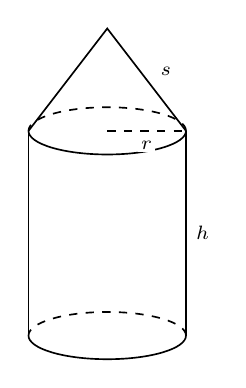
\begin{tikzpicture}[line width=0.6pt,baseline=(current bounding box.north)]\draw (-1.00,0.00) arc (180:360:1.00 and 0.30);\draw[dashed] (1.00,0.00) arc (0:180:1.00 and 0.30);\draw (-1.0,0) -- (-1.0,2.6); \draw (1.0,0) -- (1.0,2.6);\draw (-1.00,2.60) arc (180:360:1.00 and 0.30);\draw[dashed] (1.00,2.60) arc (0:180:1.00 and 0.30);\draw (-1.0,2.6) -- (0,3.9000000000000004) -- (1.0,2.6);\draw[dashed] (0,2.6) -- (1.0,2.6);\node[font=\scriptsize,right] at (1.0,1.3) {$h$};\node[font=\scriptsize,below,fill=white,inner sep=1pt] at (0.5,2.52) {$r$};\node[font=\scriptsize,right] at (0.55,3.35) {$s$};\end{tikzpicture}\par
\rechenplatz{1}
\end{pfaufg}
\begin{pfaufg}{BY ’24}{9.}{}
Ein Zylinder hat die Höhe 8 und als Grundfläche einen Kreis mit Radius 3. Kreuze den Term an, der sein Volumen angibt: 6$\pi$; 12$\pi$; 24$\pi$; 48$\pi$; 56$\pi$; 72$\pi$.
\fusshilfe{\mbox{9:~72$\pi$ (V = $\pi$ · 3² · 8)}}
\end{pfaufg}
\begin{pfaufg}{NRW ’23}{10.}{}
Karina kauft eine Glaspyramide mit quadratischer Grundfläche. Die Grundkante ist 4 cm lang, die Pyramide 6 cm hoch. Bestätige, dass ihr Volumen 32 cm³ ist.
\rechenplatz{1}
\fusshilfe{\mbox{10:~V = $\tfrac{1}{3}$ · 4² · 6 cm³ = 32 cm³}}
\end{pfaufg}
\begin{pfaufg}{BW ’22}{11.}{}
Ein Quader ist 2 m lang, 1 m breit und 1,5 m hoch. Er wird ganz mit Würfeln von je 1 dm³ gefüllt. Wie viele Würfel brauchst du?
\par\smallskip\noindent 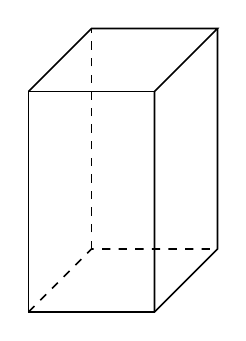
\begin{tikzpicture}[line width=0.6pt,baseline=(current bounding box.north)]\draw (0,0) rectangle (1.6,2.8); \draw (0,2.8) -- (0.8,3.5999999999999996) -- (2.4000000000000004,3.5999999999999996) -- (1.6,2.8) -- (1.6,0);\draw (2.4000000000000004,3.5999999999999996) -- (2.4000000000000004,0.8) -- (1.6,0);\draw[dashed] (0,0) -- (0.8,0.8) -- (2.4000000000000004,0.8); \draw[dashed] (0.8,0.8) -- (0.8,3.5999999999999996);\end{tikzpicture}\par
\rechenplatz{2}
\fusshilfe{\mbox{11:~3 000 dm³)}}
\end{pfaufg}
\begin{pfaufg}{}{12.}{}
Die Grundfläche eines Prismas ist ein Rechteck mit $7$ cm × $3$ cm. Das Prisma ist $5$ cm hoch. Berechne sein Volumen.
\par\noindent Grundfläche \leerfeld[cm²] , Volumen \leerfeld[cm³] \par
\fusshilfe{\mbox{12:~$105$ cm³}}
\end{pfaufg}
\begin{pfaufg}{}{13.}{}
Ein Keil liegt auf dem Boden. Vorn ist ein rechtwinkliges Dreieck, $90$ cm lang und $20$ cm hoch. Der Keil ist $70$ cm breit. Berechne sein Volumen.
\par\noindent \leerfeld[cm³] \par
\fusshilfe{\mbox{13:~$63\,000$ cm³}}
\end{pfaufg}
\pfgruppe{}
\begin{pfaufg}{SH ’23}{14.}{}
Unter einem Pool muss auf einer Fläche von 6,50 m × 4,50 m die Erde 30 cm tief ausgetauscht werden. Berechne, wie viel m³ Erde das sind.
\rechenplatz{1}
\fusshilfe{\mbox{14:~V = 6,5 · 4,5 · 0,3 $\approx$ 8,8 m³}}
\end{pfaufg}
\pfgruppe{}
\begin{pfaufg}{}{15.}{}
Ein Wasserball hat den Radius $15$ cm. Wie viel Liter Luft sind darin?
\par\noindent \leerfeld[l] \par
\fusshilfe{\mbox{15:~$\tfrac{9 \pi}{2} \approx 14{,}1$ l}}
\end{pfaufg}
\pfgruppe{}
\begin{pfaufg}{nach P10 ’23}{16.}{}
Eine zylinderförmige Dose hat innen den Radius $3{,}5$ cm und die Höhe $9$ cm. Der Hersteller gibt „ca. 350 ml“ an. Weise nach, dass die Angabe stimmt. Es gilt $1$ cm³ $= 1$ ml.
\rechenplatz{2}
\fusshilfe{\mbox{16:~das sind etwa $350$ ml}}
\end{pfaufg}
\begin{pfaufg}{}{17.}{}
Ein Kochtopf ist innen ein Zylinder mit Radius $11$ cm und Höhe $14$ cm. Wie viele Liter passen in den Topf? Runde auf eine Stelle nach dem Komma.
\par\noindent \leerfeld[l] \par
\fusshilfe{\mbox{17:~$\approx 5{,}3$ l}}
\end{pfaufg}
\begin{pfaufg}{}{18.}{}
Ein Trichter hat innen die Form eines Kegels. Der Radius ist $6$ cm, die Höhe ist $11$ cm. Wie viel Milliliter passen in den Trichter?
\par\noindent \leerfeld[ml] \par
\fusshilfe{\mbox{18:~$\approx 415$ ml}}
\end{pfaufg}
\begin{pfaufg}{P10 ’14}{19.}{2 BE}
Für ein Café wird eine Kühlvitrine in Form eines Prismas gebaut. Die Grundfläche ist ein gleichschenkliges Trapez mit den parallelen Seiten 110 cm und 80 cm, den Schenkeln 57 cm und dem Flächeninhalt 5 225 cm². Die Vitrine ist 165 cm hoch. Berechne das Volumen der Vitrine.
\par\smallskip\noindent \begin{tikzpicture}[line width=0.6pt,baseline=(current bounding box.north)]\draw (-1.50,3.70) -- (1.50,3.70) -- (1.09,2.80) -- (-1.09,2.80) -- cycle;\draw (1.50,0.90) -- (1.09,0.00) -- (-1.09,0.00) -- (-1.50,0.90);\draw[dashed] (-1.50,0.90) -- (1.50,0.90);\draw[dashed] (-1.50,0.90) -- (-1.50,3.70);\draw (1.50,0.90) -- (1.50,3.70);\draw (1.09,0.00) -- (1.09,2.80);\draw (-1.09,0.00) -- (-1.09,2.80);\path (-1.50,3.70) -- node[font=\scriptsize,above] {110} (1.50,3.70);\path (-1.09,0.00) -- node[font=\scriptsize,below] {80} (1.09,0.00);\path (1.09,2.80) -- node[font=\scriptsize,right] {57} (1.50,3.70);\path (1.09,0.00) -- node[font=\scriptsize,right] {165} (1.09,2.80);\node[font=\scriptsize,mbgrau,anchor=north west] at (-2,-0.4) {Maße in cm};\node[font=\scriptsize,mbgrau,anchor=north west] at ([yshift=-2pt]current bounding box.south west) {nicht maßstabsgerecht};\end{tikzpicture}\par
\rechenplatz{1}
\fusshilfe{\mbox{19:~862 125 cm³ ($\approx$ 0,86 m³)}}
\end{pfaufg}
\pfgruppe{}
\begin{pfaufg}{P10 ’16}{20.}{3 BE}
Eine Kugel zum Kugelstoßen hat einen Durchmesser von 12 cm. Berechne ihr Volumen.
\rechenplatz{2}
\fusshilfe{\mbox{20:~288$\pi$ $\approx$ 904,8 cm³}}
\end{pfaufg}
\pfgruppe{}
\begin{pfaufg}{P10 ’22}{21.}{2 BE}
Ein Becher hat die Form eines Zylinders ohne Deckel. Er ist h = 7 cm hoch und hat den Radius r = 3,2 cm. Zeige, dass 200 ml Flüssigkeit in den Becher passen (1 cm³ = 1 ml).
\par\smallskip\noindent \begin{tikzpicture}[line width=0.6pt,baseline=(current bounding box.north)]\fill[black!15] (-1.1,0) arc (180:360:1.1 and 0.33) -- (1.1,2.4) arc (0:-180:1.1 and 0.33) -- cycle;\draw (-1.10,0.00) arc (180:360:1.10 and 0.33);\draw[dashed] (1.10,0.00) arc (0:180:1.10 and 0.33);\draw (-1.1,0) -- (-1.1,2.4); \draw (1.1,0) -- (1.1,2.4);\draw (0,2.4) ellipse (1.1 and 0.33);\node[font=\scriptsize,mbgrau,anchor=north west] at ([yshift=-2pt]current bounding box.south west) {nicht maßstabsgerecht};\end{tikzpicture}\par
\rechenplatz{2}
\fusshilfe{\mbox{21:~71,68$\pi$ $\approx$ 225,2 cm³ > 200 ml}}
\end{pfaufg}
\pfgruppe{}
\begin{pfaufg}{P10 ’23}{22.}{2 BE}
Eine Konservendose hat die Form eines Zylinders mit dem Radius 4 cm und der Höhe 8 cm. Auf der Dose steht: Inhalt etwa 400 ml. Weise nach, dass das stimmt (1 cm³ = 1 ml).
\par\smallskip\noindent \begin{tikzpicture}[line width=0.6pt,baseline=(current bounding box.north)]\draw (-1.10,0.00) arc (180:360:1.10 and 0.33);\draw[dashed] (1.10,0.00) arc (0:180:1.10 and 0.33);\draw (-1.1,0) -- (-1.1,2.4); \draw (1.1,0) -- (1.1,2.4);\draw (0,2.4) ellipse (1.1 and 0.33);\node[font=\scriptsize,mbgrau,anchor=north west] at ([yshift=-2pt]current bounding box.south west) {nicht maßstabsgerecht};\end{tikzpicture}\par
\rechenplatz{2}
\fusshilfe{\mbox{22:~wahr, V = $\pi$ · 4² · 8 = 128$\pi$ $\approx$ 402,1 cm³ $\approx$ 400 ml}}
\end{pfaufg}
\pfgruppe{}
\begin{pfaufg}{P10 ’21}{23.}{2 BE}
Herr Gärtner stellt eine Regentonne in Form eines Zylinders auf. Sie ist h = 95 cm hoch und hat den Radius r = 29 cm. Der Hersteller gibt an, dass etwa 250 Liter Wasser in die Tonne passen. Bestätige diese Angabe mit einer Rechnung (1 l = 1 dm³).
\par\smallskip\noindent \begin{tikzpicture}[line width=0.6pt,baseline=(current bounding box.north)]\draw (-1.10,0.00) arc (180:360:1.10 and 0.33);\draw[dashed] (1.10,0.00) arc (0:180:1.10 and 0.33);\draw (-1.1,0) -- (-1.1,2.4); \draw (1.1,0) -- (1.1,2.4);\draw (0,2.4) ellipse (1.1 and 0.33);\draw (-1.1,0.7) arc (180:360:1.1 and 0.33);\draw (-1.1,1.7) arc (180:360:1.1 and 0.33);\node[font=\scriptsize,mbgrau,anchor=north west] at ([yshift=-2pt]current bounding box.south west) {nicht maßstabsgerecht};\end{tikzpicture}\par
\rechenplatz{2}
\fusshilfe{\mbox{23:~V = $\pi$ · 29² · 95 $\approx$ 250 998 cm³ $\approx$ 251 l}}
\end{pfaufg}
\pfsteckt{steckt auch in Nr. 51 (P10 ’24)}
\pfstufekopf[snetzerkennen]{Netz erkennen}{in 1 der letzten 5 Prüfungen}
\pfgruppe{}
\begin{pfaufg}{}{24.}{}
Eine Tasse ist oben $8$ cm breit, von Rand zu Rand durch die Mitte gemessen. Ist das der Radius oder der Durchmesser? Gib den Radius an.
\par\noindent Radius \leerfeld[cm] \par
\fusshilfe{\mbox{24:~Radius $4$ cm}}
\end{pfaufg}
\begin{pfaufg}{nach P10 ’17}{25.}{1 BE}
Ein Zelt hat die Form im Bild. Kreuze an, welcher Körper es ist. 
\pfkreuzzeile{Pyramide}\pfkreuzzeile{Prisma}\pfkreuzzeile{Quader}
\par\smallskip\noindent \prismadreieck{4}{2}{2.5}{}{}{}\par
\fusshilfe{\mbox{25:~Prisma}}
\end{pfaufg}
\pfgruppe{}
\begin{pfaufg}{}{26.}{}
Aus dem Netz im Bild wird ein Spielwürfel gebastelt. Auf einem Spielwürfel ergeben gegenüberliegende Augenzahlen zusammen $7$. Welche Zahlen gehören in die Felder X, Y und Z?
\par\smallskip\noindent $\begin{array}{cccc}  & 1 &  &  \\ 2 & 3 & X & Y \\  & Z &  &  \end{array}$\par
\par\noindent X = \leerfeld , Y = \leerfeld , Z = \leerfeld \par
\fusshilfe{\mbox{26:~$6$}}
\end{pfaufg}
\begin{pfaufg}{}{27.}{}
Ein Kegel hat den Radius $3$ cm und die Mantellinie $8$ cm. Sein Netz besteht aus einem Kreis und einem Kreisausschnitt. Gib den Radius des Kreises und den Radius des Kreisausschnitts an.
\par\noindent \leerfeld[cm] ; \leerfeld[cm] \par
\fusshilfe{\mbox{27:~$8$ cm}}
\end{pfaufg}
\pfgruppe{}
\begin{pfaufg}{}{28.}{}
Ein Schuhkarton hat die Form im Bild. Wie heißt dieser Körper?
\par\smallskip\noindent \quader{4}{2}{2.5}{}{}{}\par
\par\noindent \leerfeld \par
\fusshilfe{\mbox{28:~Quader}}
\end{pfaufg}
\pfgruppe{}
\begin{pfaufg}{}{29.}{}
Das Bild zeigt ein Netz. Kann man daraus einen Würfel falten? \janein
\par\smallskip\noindent $\begin{array}{cccc}  & \square &  &  \\ \square & \square & \square & \square \\  &  & \square &  \end{array}$\par
\fusshilfe{\mbox{29:~ja}}
\end{pfaufg}
\begin{pfaufg}{P10 ’17}{30.}{1 BE}
Die Abbildung zeigt einen Körper im Schrägbild. Kreuze an, welcher Körper es ist:
\pfkreuzzeile{Pyramide}\pfkreuzzeile{Prisma}\pfkreuzzeile{Quader}
\par\smallskip\noindent 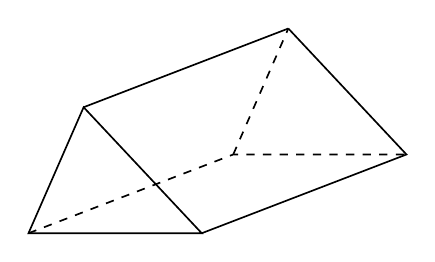
\begin{tikzpicture}[line width=0.6pt,baseline=(current bounding box.north)]\draw (0.00,0.00) -- (2.20,0.00) -- (0.70,1.60) -- cycle;\draw (3.30,2.60) -- (4.80,1.00) -- (2.20,0.00); \draw[dashed] (0.00,0.00) -- (2.60,1.00) -- (4.80,1.00);\draw (0.70,1.60) -- (3.30,2.60); \draw[dashed] (2.60,1.00) -- (3.30,2.60);\end{tikzpicture}\par
\fusshilfe{\mbox{30:~Prisma}}
\end{pfaufg}
\begin{pfaufg}{P10 ’18}{31.}{1 BE}
Kreuze an, welcher Körper zu dem abgebildeten Netz gehört:
\pfkreuzzeile{Prisma}\pfkreuzzeile{Pyramide}\pfkreuzzeile{Quader}
\par\smallskip\noindent 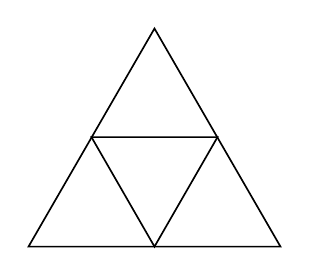
\begin{tikzpicture}[line width=0.6pt,baseline=(current bounding box.north)]\draw (0.00,0.00) -- (3.20,0.00) -- (1.60,2.77) -- cycle;\draw (1.60,0.00) -- (2.40,1.39) -- (0.80,1.39) -- cycle;\end{tikzpicture}\par
\fusshilfe{\mbox{31:~Pyramide}}
\end{pfaufg}
\pfgruppe{}
\begin{pfaufg}{P10 ’16}{32.}{1 BE}
Aus dem abgebildeten Netz wird ein Würfel gefaltet. Nach dem Falten liegt die graue Fläche oben. Markiere die Fläche, die dann unten liegt.
\par\smallskip\noindent 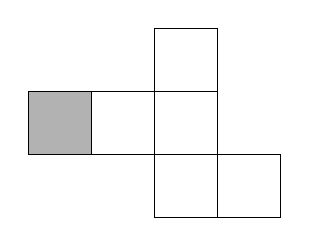
\begin{tikzpicture}[line width=0.6pt,baseline=(current bounding box.north)]\draw (1.60,1.60) rectangle ++(0.8,0.8);\draw (1.60,0.80) rectangle ++(0.8,0.8);\draw (1.60,0.00) rectangle ++(0.8,0.8);\draw (0.80,0.80) rectangle ++(0.8,0.8);\draw[fill=black!30] (0.00,0.80) rectangle ++(0.8,0.8);\draw (2.40,0.00) rectangle ++(0.8,0.8);\end{tikzpicture}\par
\rechenplatz{1}
\fusshilfe{\mbox{32:~mittleres Quadrat der senkrechten Dreierreihe}}
\end{pfaufg}
\pfgruppe{}
\begin{pfaufg}{}{33.}{}
Ein Zylinder hat den Radius $2$ cm und die Höhe $5$ cm. Kreuze an, welches Rechteck zu seinem Netz gehört. 
\pfkreuzzeile{$5$ cm × $6{,}3$ cm}\pfkreuzzeile{$5$ cm × $12{,}6$ cm}\pfkreuzzeile{$5$ cm × $4$ cm}
\fusshilfe{\mbox{33:~$4 \pi \approx 12{,}6$ cm, also $5$ cm × $12{,}6$ cm}}
\end{pfaufg}
\pfgruppe{}
\begin{pfaufg}{P10 ’22}{34.}{3 BE}
Ein Becher hat die Form eines Zylinders ohne Deckel. Er ist h = 7 cm hoch und hat den Radius r = 3,2 cm. Kreuze an, welches der drei Netze zum Becher passt. Ermittle die Länge und die Breite der Mantelfläche.
\par\smallskip\noindent 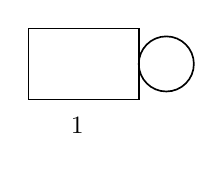
\begin{tikzpicture}[line width=0.6pt,baseline=0]\draw (0,0) rectangle (1.40,0.90); \draw (1.75,0.45) circle (0.35);\node[font=\small,anchor=north] at (0.70,-0.1) {1\enspace$\square$};\end{tikzpicture}\hspace{0.7cm}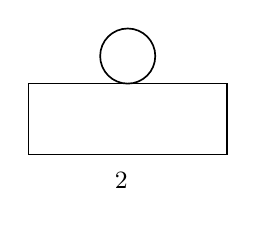
\begin{tikzpicture}[line width=0.6pt,baseline=0]\draw (0,0) rectangle (2.52,0.90); \draw (1.26,1.25) circle (0.35);\node[font=\small,anchor=north] at (1.26,-0.1) {2\enspace$\square$};\end{tikzpicture}\hspace{0.7cm}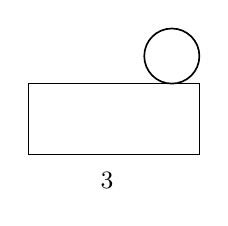
\begin{tikzpicture}[line width=0.6pt,baseline=0]\draw (0,0) rectangle (2.17,0.90); \draw (1.82,1.25) circle (0.35);\node[font=\small,anchor=north] at (1.08,-0.1) {3\enspace$\square$};\end{tikzpicture}\par
\rechenplatz{2}
\fusshilfe{\mbox{34:~drittes Netz; Länge 6,4$\pi$ $\approx$ 20,1 cm, Breite 7 cm}}
\end{pfaufg}
\pfstufekopf[srckwrtsradiusoderhhe]{rückwärts: Radius oder Höhe aus Volumen}{in 2 der letzten 5 Prüfungen}
\pfgruppe{}
\begin{pfaufg}{}{35.}{}
Eine Strecke geht von der Spitze eines Kegels zum Rand des Grundkreises. Kreuze an, wie diese Strecke heißt.
\pfkreuzzeile{Höhe}\pfkreuzzeile{Mantellinie}\pfkreuzzeile{Radius}
\fusshilfe{\mbox{35:~Mantellinie}}
\end{pfaufg}
\begin{pfaufg}{}{36.}{}
Die Figur zeigt das Netz einer Pyramide. Eine Strecke ist mit ? markiert. Kreuze an, wie diese Strecke heißt.
\pfkreuzzeile{Höhe}\pfkreuzzeile{Seitenhöhe}\pfkreuzzeile{Seitenkante}
\par\smallskip\noindent \netzpyramide{2.5}{2}{}{?}\par
\fusshilfe{\mbox{36:~Seitenhöhe}}
\end{pfaufg}
\pfgruppe{}
\begin{pfaufg}{}{37.}{}
Ein Quader hat das Volumen $90$ cm³. Er ist $5$ cm lang und $3$ cm breit. Wie hoch ist der Quader?
\par\noindent \leerfeld[cm] \par
\fusshilfe{\mbox{37:~$6$ cm}}
\end{pfaufg}
\pfgruppe{}
\begin{pfaufg}{}{38.}{}
Ein Kochtopf ist innen $200$ mm weit und $15$ cm hoch. Man gießt $3$ Liter Wasser hinein. Wie hoch steht das Wasser?
\par\noindent h $\approx$ \leerfeld[cm] \par
\fusshilfe{\mbox{38:~$3\,000 : (\pi \cdot 10^2) \approx 9{,}5$ cm}}
\end{pfaufg}
\begin{pfaufg}{nach P10 ’22}{\llap{\textasteriskcentered\,}39.}{}
Ein Eimer soll bei $15$ cm Höhe $2\,000$ cm³ fassen. Berechne den Radius. Runde auf eine Stelle nach dem Komma.
\par\noindent \leerfeld[cm] \par
\fusshilfe{\mbox{39:~$\approx 6{,}5$ cm}}
\end{pfaufg}
\pfgruppe{}
\begin{pfaufg}{P10 ’23}{\llap{\textasteriskcentered\,}40.}{3 BE}
Eine Konservendose hat die Form eines Zylinders mit dem Radius 4 cm und der Höhe 8 cm. Mit denselben Deckeln (r = 4 cm) soll auch eine größere Dose mit 1 Liter Inhalt gebaut werden. Ermittle ihre Höhe.
\par\smallskip\noindent \begin{tikzpicture}[line width=0.6pt,baseline=(current bounding box.north)]\draw (-1.10,0.00) arc (180:360:1.10 and 0.33);\draw[dashed] (1.10,0.00) arc (0:180:1.10 and 0.33);\draw (-1.1,0) -- (-1.1,2.4); \draw (1.1,0) -- (1.1,2.4);\draw (0,2.4) ellipse (1.1 and 0.33);\node[font=\scriptsize,mbgrau,anchor=north west] at ([yshift=-2pt]current bounding box.south west) {nicht maßstabsgerecht};\end{tikzpicture}\par
\rechenplatz{2}
\fusshilfe{\mbox{40:~h = 125/(2$\pi$) $\approx$ 19,9 cm}}
\end{pfaufg}
\pfgruppe{}
\begin{pfaufg}{P10 ’22}{\llap{\textasteriskcentered\,}41.}{3 BE}
Ein Becher hat die Form eines Zylinders ohne Deckel. Er ist h = 7 cm hoch und hat den Radius r = 3,2 cm. Ein größerer Becher soll 425 ml fassen und wieder 7 cm hoch sein. Berechne seinen Radius.
\par\smallskip\noindent \begin{tikzpicture}[line width=0.6pt,baseline=(current bounding box.north)]\fill[black!15] (-1.1,0) arc (180:360:1.1 and 0.33) -- (1.1,2.4) arc (0:-180:1.1 and 0.33) -- cycle;\draw (-1.10,0.00) arc (180:360:1.10 and 0.33);\draw[dashed] (1.10,0.00) arc (0:180:1.10 and 0.33);\draw (-1.1,0) -- (-1.1,2.4); \draw (1.1,0) -- (1.1,2.4);\draw (0,2.4) ellipse (1.1 and 0.33);\node[font=\scriptsize,mbgrau,anchor=north west] at ([yshift=-2pt]current bounding box.south west) {nicht maßstabsgerecht};\end{tikzpicture}\par
\rechenplatz{3}
\fusshilfe{\mbox{41:~r = √(425/(7$\pi$)) $\approx$ 4,40 cm}}
\end{pfaufg}
\pfstufekopf[srestvolumen]{Restvolumen}{in 1 der letzten 5 Prüfungen}
\pfgruppe{}
\begin{pfaufg}{}{42.}{}
Ein Ball passt genau in eine Schachtel. Die Schachtel ist $22$ cm breit. Kreuze an, ob die $22$ cm der Radius oder der Durchmesser des Balls sind.
\pfkreuzzeile{Radius}\pfkreuzzeile{Durchmesser}
\fusshilfe{\mbox{42:~Durchmesser}}
\end{pfaufg}
\begin{pfaufg}{}{43.}{}
Ein Haus hat ein Satteldach. Aus welchen zwei Körpern besteht das Haus?
\rechenplatz{3}
\fusshilfe{\mbox{43:~Quader und Dreiecksprisma}}
\end{pfaufg}
\pfgruppe{}
\begin{pfaufg}{}{44.}{}
Eine Betonstufe besteht aus zwei Quadern. Der untere misst $8$ dm × $4$ dm × $2$ dm. Darauf liegt einer mit $8$ dm × $2$ dm × $2$ dm. Berechne das Volumen der Stufe.
\par\noindent \leerfeld[dm³] \par
\fusshilfe{\mbox{44:~$96$ dm³}}
\end{pfaufg}
\begin{pfaufg}{BW ’23}{45.}{}
Aus einem Quader (5 cm × 10 cm × 3 cm) sind zwei Leisten von je 1 cm × 10 cm × 1 cm herausgeschnitten. Berechne das Volumen des Körpers.
\par\smallskip\noindent 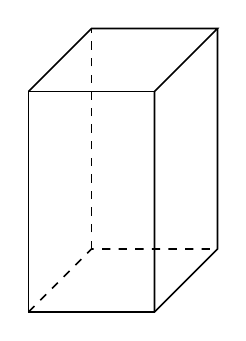
\begin{tikzpicture}[line width=0.6pt,baseline=(current bounding box.north)]\draw (0,0) rectangle (1.6,2.8); \draw (0,2.8) -- (0.8,3.5999999999999996) -- (2.4000000000000004,3.5999999999999996) -- (1.6,2.8) -- (1.6,0);\draw (2.4000000000000004,3.5999999999999996) -- (2.4000000000000004,0.8) -- (1.6,0);\draw[dashed] (0,0) -- (0.8,0.8) -- (2.4000000000000004,0.8); \draw[dashed] (0.8,0.8) -- (0.8,3.5999999999999996);\end{tikzpicture}\par
\rechenplatz{2}
\fusshilfe{\mbox{45:~130 cm³ (150 $-$ 2 · 10)}}
\end{pfaufg}
\pfgruppe{}
\begin{pfaufg}{}{46.}{}
Ein Kupferrohr ist $3$ m lang. Außen misst es $22$ mm im Durchmesser, die Wand ist $1$ mm dick. Kupfer wiegt $8{,}9$ g pro cm³. Wie schwer ist das Rohr?
\par\noindent m $\approx$ \leerfeld[kg] \par
\fusshilfe{\mbox{46:~$\approx 1{,}76$ kg}}
\end{pfaufg}
\begin{pfaufg}{}{47.}{2 BE}
Aus einem Holzwürfel mit der Kante $12$ cm wird die größte Kugel gedrechselt. a) Berechne das Volumen der Kugel. b) Wie viel Prozent des Holzes fallen ab? c) Begründe, dass bei jedem Würfel derselbe Anteil abfällt.
\par\noindent a) \leerfeld[cm³]   b) \leerfeld[\%] \par
\fusshilfe{\mbox{47:~$a : 2$, die Kugel hat $\tfrac{\pi}{6} \cdot a^3$}}
\end{pfaufg}
\begin{pfaufg}{NI ’23}{48.}{}
Ein kugelförmiger Gasspeicher hat außen 27 m Durchmesser. Seine Metallwand ist 0,03 m dick. Berechne das Volumen innen.
\rechenplatz{2}
\fusshilfe{\mbox{48:~13,47 m; $\approx$ 10 237,44 m³}}
\end{pfaufg}
\begin{pfaufg}{NRW ’22}{49.}{}
Herr Paulsen kauft 130 Bambusrohre, je 180 cm lang, mit 7,1 cm² Querschnitt aus Holz. 1 cm³ Bambusholz wiegt 0,7 g. Sein Anhänger trägt 250 kg. Berechne das Gewicht der Rohre und entscheide, ob der Anhänger reicht.
\rechenplatz{3}
\fusshilfe{\mbox{49:~1 278 cm³ je Rohr; $\approx$ 116 kg < 250 kg: reicht}}
\end{pfaufg}
\begin{pfaufg}{}{50.}{}
Ein Tortenkarton ist innen $24$ cm × $24$ cm × $9$ cm groß. Darin steht eine runde Torte mit $22$ cm Durchmesser und $8$ cm Höhe. Wie viel Luft bleibt im Karton? Runde auf eine Stelle nach dem Komma.
\par\noindent \leerfeld[cm³] \par
\fusshilfe{\mbox{50:~$2\,142{,}9$ cm³}}
\end{pfaufg}
\pfgruppe{}
\begin{pfaufg}{P10 ’24}{\llap{\textasteriskcentered\,}51.}{3 BE}
Eine Firma stellt Kegel mit dem Radius r = 30 cm und der Höhe h = 80 cm her. Eine andere Firma verschickt denselben Kegel in einer zylinderförmigen Verpackung; innen ist sie 81 cm hoch und hat den Radius 30,5 cm. Der freie Raum wird mit Füllmaterial ausgefüllt. Ermittle, wie viele cm³ Füllmaterial man braucht.
\par\smallskip\noindent \begin{tikzpicture}[line width=0.6pt,baseline=(current bounding box.north)]\fill[black!15] (0,0) ellipse (1.2 and 0.36);\draw (-1.20,0.00) arc (180:360:1.20 and 0.36);\draw[dashed] (1.20,0.00) arc (0:180:1.20 and 0.36);\draw (-1.2,0) -- (0,2.4) -- (1.2,0);\node[font=\scriptsize,mbgrau,anchor=north west] at ([yshift=-2pt]current bounding box.south west) {nicht maßstabsgerecht};\end{tikzpicture}\par
\rechenplatz{3}
\fusshilfe{\mbox{51:~51 350,25$\pi$ $\approx$ 161 322 cm³}}
\end{pfaufg}
\pfstufekopf[smantelflchemitkosten]{Mantelfläche mit Kosten}{in 1 der letzten 5 Prüfungen}
\pfgruppe{}
\begin{pfaufg}{}{52.}{}
Eine Tonne hat den Durchmesser $0{,}5$ m und die Höhe $70$ cm. Schreibe vor dem Rechnen beide Maße in cm.
\par\noindent \leerfeld[cm]  und \leerfeld[cm] \par
\fusshilfe{\mbox{52:~$50$ cm und $70$ cm}}
\end{pfaufg}
\begin{pfaufg}{}{53.}{}
Die Figur zeigt ein Turmdach in Form einer Pyramide. Zeichne das rechtwinklige Dreieck aus Höhe, halber Grundkante und Seitenhöhe ein. Markiere die Hypotenuse. Du musst nichts rechnen.
\par\smallskip\noindent \pyramide{4}{4}{3}{$6$ m}{}{$4$ m}\par
\rechenplatz{2}
\end{pfaufg}
\pfgruppe{}
\begin{pfaufg}{NI ’23}{54.}{}
Eine quadratische Pyramide hat die Grundkante 7 cm und die Seitenhöhe 8,73 cm. Berechne ihre Mantelfläche.
\rechenplatz{1}
\fusshilfe{\mbox{54:~M = 4 · ½ · 7 · 8,73 cm² = 122,22 cm²}}
\end{pfaufg}
\begin{pfaufg}{nach NI ’26}{55.}{}
Eine geschlossene Taschentuchbox ist 25 cm lang, 11 cm breit und 9 cm hoch. Berechne ihre Oberfläche.
\rechenplatz{1}
\fusshilfe{\mbox{55:~O = 2 · (275 + 225 + 99) cm² = 1 198 cm²}}
\end{pfaufg}
\pfgruppe{}
\begin{pfaufg}{}{56.}{}
Ein Zylinder hat den Radius $4$ cm und die Höhe $9$ cm. Berechne seinen Mantel. Runde auf eine Stelle nach dem Komma.
\par\noindent \leerfeld[cm²] \par
\fusshilfe{\mbox{56:~$72 \pi \approx 226{,}2$ cm²}}
\end{pfaufg}
\begin{pfaufg}{}{57.}{}
Ein Kegel hat den Radius $4$ cm und die Mantellinie $11$ cm. Berechne den Flächeninhalt des Mantels. Runde auf eine Stelle nach dem Komma.
\par\noindent $M$ $\approx$ \leerfeld[cm²] \par
\fusshilfe{\mbox{57:~$\pi \cdot 4 \cdot 11 \approx 138{,}2$ cm²}}
\end{pfaufg}
\pfgruppe{}
\begin{pfaufg}{P10 ’18}{58.}{2 BE}
Ein runder Turm hat 6,4 m Durchmesser. Seine zylinderförmige Außenmauer ist 21,7 m hoch und soll renoviert werden. Berechne die Fläche der Außenmauer.
\rechenplatz{2}
\fusshilfe{\mbox{58:~138,88$\pi$ $\approx$ 436,3 m²}}
\end{pfaufg}

\par\Needspace*{0.55\textheight}\pfstufekopf[serkennen1]{Was ist gesucht?}{}
\begin{pfaufg}{}{59.}{}
Was ist gesucht? Kreuze an. Rechne nicht.
\par\smallskip\noindent \begingroup\renewcommand{\arraystretch}{1.4}\begin{tabular}{|>{\raggedright\arraybackslash}p{8.3cm}|>{\centering\arraybackslash\hyphenpenalty=0}p{1.55cm}|>{\centering\arraybackslash\hyphenpenalty=0}p{1.55cm}|}\hline  & {\scriptsize\hspace{0pt}Mantelfläche mit Kosten} & {\scriptsize\hspace{0pt}Volumen direkt} \\ \hline Reicht ein Karton von 11 cm × 15 cm für die Mäntel von Hut und Rumpf der Puppe? & $\square$ & $\square$ \\ \hline Ein Würfel hat die Kantenlänge 3 cm. Wie groß ist sein Rauminhalt? & $\square$ & $\square$ \\ \hline Die Außenmauer eines runden Turms (d = 6,4 m, 21,7 m hoch) wird gestrichen. Wie groß ist die Fläche? & $\square$ & $\square$ \\ \hline Eine Dose hat den Radius 4 cm und ist 8 cm hoch. Passen 400 ml hinein? & $\square$ & $\square$ \\ \hline Ein Kegeldach (r = 4,7 m, s = 8,6 m) wird mit Ziegeln gedeckt, 1 m² kostet 20 €. Was kosten die Ziegel? & $\square$ & $\square$ \\ \hline Ein Becher ist 7 cm hoch und hat den Radius 3,2 cm. Passen 200 ml hinein? & $\square$ & $\square$ \\ \hline\end{tabular}\endgroup\par
\end{pfaufg}
\pfstufekopf[svergleichenundurteil]{vergleichen und urteilen}{in 1 der letzten 5 Prüfungen}
\pfgruppe{}
\begin{pfaufg}{}{60.}{}
Eine Eistüte ist oben $6$ cm breit. Entscheide, ob das der Radius oder der Durchmesser ist. Gib dann die andere Größe an.
\par\noindent \leerfeld \par
\fusshilfe{\mbox{60:~$3$ cm}}
\end{pfaufg}
\pfgruppe{}
\begin{pfaufg}{NI ’23}{61.}{}
Ein zweiter kugelförmiger Gasspeicher hat den doppelten Durchmesser. Begründe, dass sein Volumen achtmal so groß ist.
\rechenplatz{1}
\fusshilfe{\mbox{61:~V ~ r³, 2³ = 8}}
\end{pfaufg}
\begin{pfaufg}{SH ’24}{62.}{}
Lisa verdoppelt alle Kantenlängen eines Holzquaders. Sie meint: Dann verdoppelt sich auch das Volumen. Entscheide, ob Lisa recht hat, und begründe.
\rechenplatz{1}
\fusshilfe{\mbox{62:~Nein}}
\end{pfaufg}
\begin{pfaufg}{SH ’25}{63.}{}
Aus gleich großen Knetzylindern soll ein großer Zylinder entstehen. Er hat den dreifachen Radius und dieselbe Höhe. Gib an, wie viele kleine Zylinder man braucht.
\fusshilfe{\mbox{63:~V ~ r²: 3² = 9 Stück}}
\end{pfaufg}
\begin{pfaufg}{NI ’26}{64.}{}
Der Radius eines Kegels wird verdoppelt, die Höhe bleibt. Wie ändert sich sein Volumen? Verdoppelt, verdreifacht oder vervierfacht? Kreuze an.
\fusshilfe{\mbox{64:~vervierfacht (V ~ r²)}}
\end{pfaufg}
\begin{pfaufg}{NRW ’23}{65.}{}
Elon sagt: „Wenn ich die Höhe des Quaders verdopple, vervierfacht sich sein Volumen.“ Hat Elon recht? Begründe.
\rechenplatz{1}
\fusshilfe{\mbox{65:~a · b · 2c)}}
\end{pfaufg}
\pfgruppe{}
\begin{pfaufg}{}{66.}{}
Der Radius eines Zylinders wird verdoppelt. Erkläre, warum das Volumen dann viermal so groß wird.
\rechenplatz{1}
\end{pfaufg}
\begin{pfaufg}{}{67.}{}
Ein Kegel und ein Zylinder haben gleichen Radius und gleiche Höhe. Begründe, warum man den Kegel dreimal füllen muss, bis der Zylinder voll ist.
\rechenplatz{1}
\end{pfaufg}
\pfgruppe{}
\begin{pfaufg}{}{68.}{}
Kugel A hat den Radius $2$ cm. Kugel B hat den Radius $4$ cm. Berechne beide Volumen. Zeige damit, dass Kugel B achtmal so viel Volumen hat.
\rechenplatz{3}
\fusshilfe{\mbox{68:~das Achtfache, weil $2^3 = 8$}}
\end{pfaufg}
\pfgruppe{}
\begin{pfaufg}{P10 ’21}{\llap{\textasteriskcentered\,}69.}{2 BE}
Herr Gärtner stellt eine Regentonne in Form eines Zylinders auf. Sie ist h = 95 cm hoch und hat den Radius r = 29 cm. Herr Gärtner meint: „Eine Tonne mit doppeltem Radius würde genau doppelt so viel Wasser fassen.“ Entscheide, ob das stimmt. Begründe deine Entscheidung.
\par\smallskip\noindent \begin{tikzpicture}[line width=0.6pt,baseline=(current bounding box.north)]\draw (-1.10,0.00) arc (180:360:1.10 and 0.33);\draw[dashed] (1.10,0.00) arc (0:180:1.10 and 0.33);\draw (-1.1,0) -- (-1.1,2.4); \draw (1.1,0) -- (1.1,2.4);\draw (0,2.4) ellipse (1.1 and 0.33);\draw (-1.1,0.7) arc (180:360:1.1 and 0.33);\draw (-1.1,1.7) arc (180:360:1.1 and 0.33);\node[font=\scriptsize,mbgrau,anchor=north west] at ([yshift=-2pt]current bounding box.south west) {nicht maßstabsgerecht};\end{tikzpicture}\par
\rechenplatz{1}
\fusshilfe{\mbox{69:~$\approx$ 1004 l)}}
\end{pfaufg}
\pfstufekopf[snetzmitmaenskizziere]{Netz mit Maßen skizzieren}{in 2 der letzten 5 Prüfungen}
\pfgruppe{}
\begin{pfaufg}{}{70.}{}
Zeichne das Netz einer Streichholzschachtel. Die Schachtel ist ein Quader. Sie ist $4$ cm lang, $2$ cm breit und $1$ cm hoch.
\par\smallskip\noindent \rechenplatz{5}\par
\rechenplatz{2}
\end{pfaufg}
\begin{pfaufg}{}{71.}{}
Das Bild zeigt ein Prisma. Das Dreieck ist gleichschenklig, die Schenkel sind je $5$ cm lang. Skizziere das Netz des Prismas mit allen Maßen.
\par\smallskip\noindent \prismadreieck{4}{1.5}{2.5}{$8$ cm}{$3$ cm}{$7$ cm} \rechenplatz[halb]{4}\par
\rechenplatz{1}
\fusshilfe{\mbox{71:~zwei Dreiecke mit den Seiten $8$ cm, $5$ cm, $5$ cm}}
\end{pfaufg}
\begin{pfaufg}{P10 ’20}{72.}{2 BE}
Eine Schachtel hat die Form eines Prismas. Ihre Grundfläche ist ein Rechteck, 14 cm breit und 12 cm tief. Die vordere Kante ist 6 cm hoch, die hintere 15 cm; die Deckfläche verläuft schräg und ist etwa 16 cm breit. Die beiden Seitenflächen sind Trapeze mit zwei rechten Winkeln. Ein Netz ist schon begonnen. Vervollständige das Netz.
\par\smallskip\noindent \begin{tikzpicture}[line width=0.6pt,baseline=(current bounding box.north)]\draw (0,0) -- (2.8,0) -- (2.8,1.2) -- (0,1.2) -- cycle;\draw (2.8,0) -- (3.6,0.5) -- (3.6,3.5) -- (2.8,1.2);\draw (0,1.2) -- (0.8,3.5) -- (3.6,3.5);\draw[dashed] (0,0) -- (0.8,0.5) -- (3.6,0.5); \draw[dashed] (0.8,0.5) -- (0.8,3.5);\path (0.00,0.00) -- node[font=\scriptsize,below] {14 cm} (2.80,0.00);\path (2.80,0.00) -- node[font=\scriptsize,below right] {12 cm} (3.60,0.50);\path (0.00,0.00) -- node[font=\scriptsize,left] {6 cm} (0.00,1.20);\path (3.60,0.50) -- node[font=\scriptsize,right] {15 cm} (3.60,3.50);\path (0.00,1.20) -- node[font=\scriptsize,left] {16 cm} (0.80,3.50);\draw[mbgitter,line width=0.3pt,step=0.25] (5,-0.5) grid (10.5,3.25);\draw (5.250,0) rectangle ++(2.075,1.500);\draw (7.325,0) rectangle ++(0.750,1.500);\draw (8.075,0) rectangle ++(1.750,1.500);\draw (8.075,1.500) -- (8.075,2.250) -- (9.825,3.375) -- (9.825,1.500);\node[font=\scriptsize,mbgrau,anchor=north west] at (5,-0.5) {1 Kästchen = 2 cm};\node[font=\scriptsize,mbgrau,anchor=north west] at ([yshift=-2pt]current bounding box.south west) {nicht maßstabsgerecht};\end{tikzpicture}\par
\rechenplatz{1}
\end{pfaufg}
\begin{pfaufg}{}{73.}{}
Die Figur zeigt verkleinert das Netz einer Pyramide mit einem Quadrat als Grundfläche. Die Grundkante ist $4$ cm lang, die Seitenhöhe ist $5$ cm. Zeichne in jede Seitenfläche die Seitenhöhe ein. Schreibe die Maße an die Grundkanten und an die Seitenhöhen.
\par\smallskip\noindent \netzpyramide{2}{2.5}{}{}\par
\rechenplatz{1}
\fusshilfe{\mbox{73:~alle vier Seiten des Quadrats $4$ cm}}
\end{pfaufg}
\begin{pfaufg}{HH ’26}{74.}{}
Ein Pappkarton ist ein Quader mit 20 cm, 15 cm und 10 cm Kantenlänge. Zeichne ein Netz im Maßstab 1 : 5 und bestätige, dass es 1 300 cm² groß ist.
\par\smallskip\noindent \begin{tikzpicture}[x=0.5cm,y=0.5cm]\draw[mbgitter,line width=0.3pt] (0,0) grid (28,15);\end{tikzpicture}\par
\rechenplatz{2}
\fusshilfe{\mbox{74:~1 300 cm²}}
\end{pfaufg}
\pfgruppe{}
\begin{pfaufg}{P10 ’19}{75.}{2 BE}
Auf einem Mast sitzt ein dreiseitiges Prisma. Seine drei Seitenflächen sind Rechtecke mit 1,50 m Breite und 1,20 m Höhe; Grund- und Deckfläche sind gleichseitige Dreiecke. Das Netz des Prismas ist schon begonnen. Vervollständige das Netz. Gib die Länge a an.
\par\smallskip\noindent \begin{tikzpicture}[x=0.4cm,y=0.4cm,line width=0.6pt,baseline=(current bounding box.north)]\draw[mbgitter,line width=0.3pt,step=1] (0,0) grid (26,12);\draw (2,7) rectangle ++(5,4); \draw (7,7) rectangle ++(5,4);\draw (7,7) -- (12,7) -- (9.50,2.67) -- cycle;\node[font=\small,anchor=west] at (11.00,4.83) {$a$};\end{tikzpicture}\par
\rechenplatz{1}
\fusshilfe{\mbox{75:~a = 1,50 m}}
\end{pfaufg}
\begin{pfaufg}{P10 ’14}{76.}{4 BE}
Für ein Café wird eine Kühlvitrine in Form eines Prismas gebaut. Die Grundfläche ist ein gleichschenkliges Trapez mit den parallelen Seiten 110 cm und 80 cm, den Schenkeln 57 cm und dem Flächeninhalt 5 225 cm². Die Vitrine ist 165 cm hoch. Ein Netz der Vitrine ist schon begonnen. Vervollständige das Netz. Gib die fehlenden Maße a, b und d an.
\par\smallskip\noindent 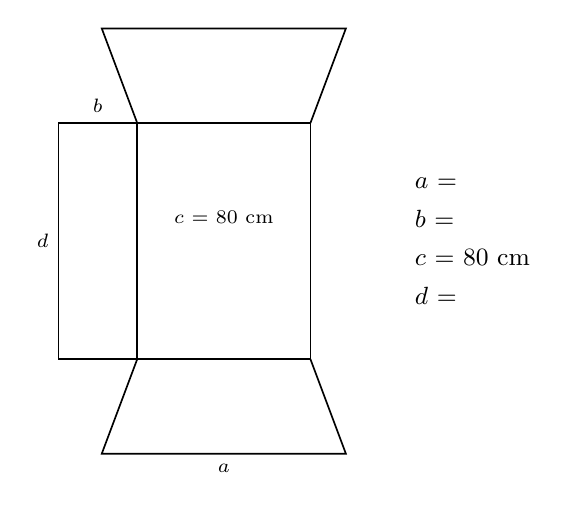
\begin{tikzpicture}[line width=0.6pt,baseline=(current bounding box.north)]\draw (0,0) rectangle (1.0,3.0); \draw (1.0,0) rectangle (3.2,3.0);\draw (1.0,3.0) -- (0.55,4.2) -- (3.6500000000000004,4.2) -- (3.2,3.0);\draw (1.0,0) -- (0.55,-1.2) -- (3.6500000000000004,-1.2) -- (3.2,0);\node[font=\scriptsize,below] at (2.1,-1.2) {$a$};\node[font=\scriptsize,above] at (0.5,3.0) {$b$};\node[font=\scriptsize] at (2.1,1.8) {$c$ = 80 cm};\node[font=\scriptsize,left] at (0,1.5) {$d$};\node[font=\small,anchor=west,align=left] at (4.4,1.5) {$a$ = \leerzelle\\[3pt] $b$ = \leerzelle\\[3pt] $c$ = 80 cm\\[3pt] $d$ = \leerzelle};\end{tikzpicture}\par
\fusshilfe{\mbox{76:~165 cm}}
\end{pfaufg}
\pfgruppe{}
\begin{pfaufg}{}{77.}{}
Aus dem Netz im Bild wird ein Zylinder gefaltet. Wie viel passt hinein? Runde auf eine Stelle nach dem Komma.
\par\smallskip\noindent \netzzylinder{1}{2.5}{$2$ cm}{$5$ cm}\par
\par\noindent \leerfeld[cm³] \par
\fusshilfe{\mbox{77:~$20 \pi \approx 62{,}8$ cm³}}
\end{pfaufg}
\pfgruppe{}
\begin{pfaufg}{P10 ’23}{78.}{3 BE}
Eine Konservendose hat die Form eines Zylinders mit dem Radius 4 cm und der Höhe 8 cm. Skizziere die Mantelfläche der Dose. Bestimme ihre Länge a und ihre Breite b und schreibe beide an deine Skizze.
\par\smallskip\noindent \begin{tikzpicture}[line width=0.6pt,baseline=(current bounding box.north)]\draw (-1.10,0.00) arc (180:360:1.10 and 0.33);\draw[dashed] (1.10,0.00) arc (0:180:1.10 and 0.33);\draw (-1.1,0) -- (-1.1,2.4); \draw (1.1,0) -- (1.1,2.4);\draw (0,2.4) ellipse (1.1 and 0.33);\node[font=\scriptsize,mbgrau,anchor=north west] at ([yshift=-2pt]current bounding box.south west) {nicht maßstabsgerecht};\end{tikzpicture}\par
\rechenplatz{2}
\fusshilfe{\mbox{78:~Rechteck, a = 8$\pi$ $\approx$ 25,1 cm, b = 8 cm}}
\end{pfaufg}
\pfsteckt{steckt auch in Nr. 34 (P10 ’22)}
\pfstufekopf[skrperimschrgbildskiz]{Körper im Schrägbild skizzieren}{in 1 der letzten 5 Prüfungen}
\pfgruppe{}
\begin{pfaufg}{}{79.}{}
Ein Quader ist $6$ cm lang, $4$ cm tief und $3$ cm hoch. Zeichne sein Schrägbild auf Kästchenpapier.
\par\smallskip\noindent \rechenplatz{5}\par
\rechenplatz{3}
\fusshilfe{\mbox{79:~Tiefe $4$ cm schräg als $2$ cm}}
\end{pfaufg}
\pfgruppe{}
\begin{pfaufg}{nach P10 ’24}{80.}{}
Ein Kegel aus Beton hat die Form eines Kegels mit Radius $25$ cm und Höhe $70$ cm. Er wird in einem quaderförmigen Karton verschickt, der so klein wie möglich ist. Skizziere den Kegel in das Schrägbild des Kartons.
\par\smallskip\noindent \quader{2.5}{2.5}{3.5}{}{}{}\par
\rechenplatz{4}
\fusshilfe{\mbox{80:~Spitze in der Mitte des Deckels}}
\end{pfaufg}
\begin{pfaufg}{}{81.}{}
Die Figur zeigt eine Pyramide mit einem Quadrat als Grundfläche. Ihre Seitenhöhe ist $7$ cm lang. Skizziere das Netz der Pyramide und schreibe die Maße an.
\par\smallskip\noindent \pyramide{4}{4}{3}{$5$ cm}{}{}\par
\rechenplatz{1}
\end{pfaufg}
\begin{pfaufg}{}{82.}{}
Eine Waffeltüte ist oben $5$ cm breit und $11$ cm tief. Skizziere die Tüte als Kegel mit der Spitze nach unten. Beschrifte den Radius und die Höhe.
\par\smallskip\noindent \rechenplatz[halb]{4}\par
\rechenplatz{2}
\end{pfaufg}
\pfgruppe{}
\begin{pfaufg}{P10 ’24}{83.}{4 BE}
Eine Firma stellt Kegel mit dem Radius r = 30 cm und der Höhe h = 80 cm her. Der Kegel soll in einem quaderförmigen Karton verschickt werden, der möglichst klein ist, in den der Kegel aber ganz hineinpasst. Skizziere den Kegel in den Karton. Kreuze die kleinste passende Größe an (Länge × Breite × Höhe):
\pfkreuzzeile{31 cm × 31 cm × 81 cm}\pfkreuzzeile{61 cm × 61 cm × 101 cm}\pfkreuzzeile{61 cm × 61 cm × 81 cm}\pfkreuzzeile{31 cm × 61 cm × 81 cm. Begründe deine Wahl}
\par\smallskip\noindent 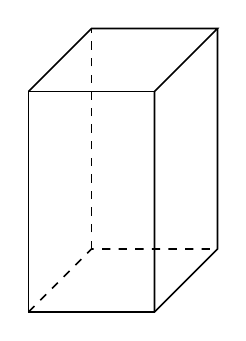
\begin{tikzpicture}[line width=0.6pt,baseline=(current bounding box.north)]\draw (0,0) rectangle (1.6,2.8); \draw (0,2.8) -- (0.8,3.5999999999999996) -- (2.4000000000000004,3.5999999999999996) -- (1.6,2.8) -- (1.6,0);\draw (2.4000000000000004,3.5999999999999996) -- (2.4000000000000004,0.8) -- (1.6,0);\draw[dashed] (0,0) -- (0.8,0.8) -- (2.4000000000000004,0.8); \draw[dashed] (0.8,0.8) -- (0.8,3.5999999999999996);\end{tikzpicture}\par
\rechenplatz{1}
\fusshilfe{\mbox{83:~61 cm × 61 cm × 81 cm}}
\end{pfaufg}
\pfgruppe{}
\begin{pfaufg}{}{84.}{}
Skizziere eine Kugel mit dem Radius $2$ cm. Zeichne einen Kreis und den Äquator als flache Ellipse. Zeichne den Radius gestrichelt ein und beschrifte ihn.
\par\smallskip\noindent \rechenplatz[halb]{4}\par
\rechenplatz{3}
\end{pfaufg}
\pfgruppe{}
\begin{pfaufg}{P10 ’15}{85.}{2 BE}
Mia hat ein Modell einer Pyramide mit quadratischer Grundfläche gebaut: Es ist 0,68 m hoch, die Grundkante ist 0,80 m lang. Zeichne in das Schrägbild die Höhe der Pyramide ein. Beschrifte die Skizze mit den gegebenen Maßen.
\par\smallskip\noindent \begin{tikzpicture}[line width=0.6pt,baseline=(current bounding box.north)]\draw (0,0) -- (2.4,0) -- (3.3,0.9);\draw[dashed] (3.3,0.9) -- (0.9,0.9) -- (0,0); \draw[dashed] (0.9,0.9) -- (1.65,2.6);\draw (0,0) -- (1.65,2.6);\draw (2.4,0) -- (1.65,2.6);\draw (3.3,0.9) -- (1.65,2.6);\node[font=\scriptsize,mbgrau,anchor=north west] at ([yshift=-2pt]current bounding box.south west) {nicht maßstabsgerecht};\end{tikzpicture}\par
\rechenplatz{1}
\fusshilfe{\mbox{85:~0,68 m; Grundkante 0,80 m}}
\end{pfaufg}
\pfpruefstein{P10 ’26}
\begin{pfaufg}{}{}{}
Ein Turm besteht unten aus einem Zylinder, sein Dach ist ein Kegel. Bekannt sind: h = 25,0 m (Höhe des Zylinders), r = 4,7 m (Radius von Zylinder und Kegel) und s = 8,6 m (Mantellinie des Kegels).
\par\smallskip\noindent \begin{tikzpicture}[line width=0.6pt,baseline=(current bounding box.north)]\draw (-1.00,0.00) arc (180:360:1.00 and 0.30);\draw[dashed] (1.00,0.00) arc (0:180:1.00 and 0.30);\draw (-1.0,0) -- (-1.0,2.6); \draw (1.0,0) -- (1.0,2.6);\draw (-1.00,2.60) arc (180:360:1.00 and 0.30);\draw[dashed] (1.00,2.60) arc (0:180:1.00 and 0.30);\draw (-1.0,2.6) -- (0,3.9000000000000004) -- (1.0,2.6);\draw[dashed] (0,2.6) -- (1.0,2.6);\node[font=\scriptsize,right] at (1.0,1.3) {$h$ = 25,0 m};\node[font=\scriptsize,below,fill=white,inner sep=1pt] at (0.5,2.52) {$r$ = 4,7 m};\node[font=\scriptsize,right] at (0.55,3.35) {$s$ = 8,6 m};\node[font=\scriptsize,mbgrau,anchor=north west] at ([yshift=-2pt]current bounding box.south west) {nicht maßstabsgerecht};\end{tikzpicture}\par
\end{pfaufg}
\begin{pfaufg}{}{a)}{2 BE}
Berechne das Volumen des zylinderförmigen Teils.
\rechenplatz{3}
\fusshilfe{\mbox{Prüfstein a):~552,25$\pi$ $\approx$ 1734,9 m³}}
\end{pfaufg}
\begin{pfaufg}{}{b)}{3 BE}
Das Dach wird mit Ziegeln gedeckt; 1 m² Ziegel kostet 20,00 €. Berechne die Kosten für die Ziegel.
\rechenplatz{3}
\fusshilfe{\mbox{Prüfstein b):~$\approx$ 2539,66 € (rund 2540 €)}}
\end{pfaufg}
\begin{pfaufg}{}{*c)}{3 BE}
Ein Turm besteht aus einem Zylinder (Höhe 25,0 m, Radius 4,7 m) mit einem Kegeldach; die Mantellinie des Kegels ist 8,6 m lang, sein Radius ebenfalls 4,7 m. Bestimme die Gesamthöhe des Turms.
\rechenplatz{3}
\fusshilfe{\mbox{Prüfstein c):~25 + √51,87 $\approx$ 32,2 m}}
\end{pfaufg}
\begin{pfaufg}{}{*d)}{3 BE}
Ein Zylinder und ein Kegel sind gleich hoch. Jemand behauptet: „Ist der Radius des Kegels dreimal so groß wie der des Zylinders, haben beide dasselbe Volumen.“ Untersuche mit einer Rechnung, ob das stimmt.
\rechenplatz{3}
\fusshilfe{\mbox{Prüfstein d):~3 · V\_Zylinder $\Rightarrow$ dreifaches Volumen}}
\end{pfaufg}
\end{document}